%%% Time-stamp: <2023-06-13 12:08:59 vladimir>
%%% Copyright (C) 2019-2023 Vladimir G. Ivanović
%%% Author: Vladimir G. Ivanović <vladimir@acm.org>
%%% ORCID: https://orcid.org/0000-0002-7802-7970

\chapter{Rocketship Property Information}\label{ch:rocketship-property-info}
\bigskip%
Each of the 10 existing Rocketship schools in Santa Clara County which were listed in \prettyref{tab:RocketshipLocations} are described in a section below. Each section comprises some basic property information, a plat map of the property, its assessed valuation over the last three years, and a satellite photograph of the school site.

Except for the photos, all of the information presented in this appendix is available from the web site of the Office of the Assessor, County of Santa Clara, under the heading ``Real Property Search'' (\url{https://tinyurl.com/assessors-office-santa-clara}).

\clearpage

%%%%%%%%%%%%%%%%%%%%%%%%%%%%%%%%%%%%%%%%%%%%%%%%%%%%%%%%%%%%%%%%%%%%%%%%%%%%%%%%%%%%%%%%%%%%%%%%%%%%%%%%%%%%%%%%%%%%%%%%%

\section{Mateo Sheedy}\label{sec:mateo-sheedy-info}
\begin{table}[htb]
  \SingleSpacing%
  \caption[Mateo Sheedy: Property Information]{\textit{Mateo Sheedy: Property Information}}\label{tab:mateo-sheedy-prop-info}
  \begin{tabular}{ll}
    \toprule
    Property Address      & 788 Locust St., San José, CA 95110 \\
    Assessor's Parcel No. &  264–34–076 \\
    Size (acres)          & 1.55 \\
    Date of Last Sale     & 11 Mar 2016 \\
    \bottomrule
  \end{tabular}
\end{table}

\begin{figure}[hbt]
    \caption[Mateo Sheedy Plat Map]{\textit{Mateo Sheedy Plat Map}}\label{fig:mateo-sheedy-plat-map}
    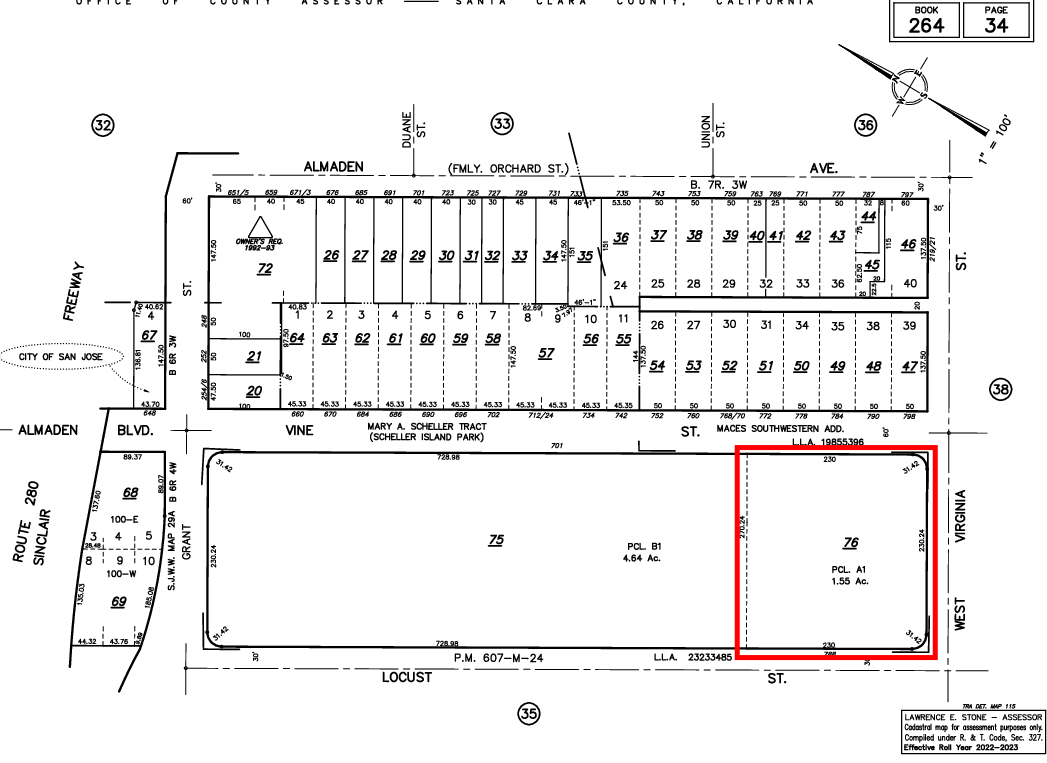
\includegraphics[width=\textwidth]{Assessor-Info/mateo-sheedy-plat-map-264-34}\\ %chktex 8
    \footnotesize{Santa Clara County Assessor's Office (n.d.). [Plat Map]. Retrieved 22 Dec 2022 from  \url{https://tinyurl.com/mateo-sheedy-plat-map}}.
\end{figure}

\begin{table}[hbt]
  \SingleSpacing%
  \caption[Mateo Sheedy: Taxable Amount of Assessed Propery]{\textit{Mateo Sheedy: Taxable Amount of Assessed Property}}\label{tab:mateo-sheedy-taxable-amount}
  \begin{tabular}{llll}
    \toprule
    Year & Land        & Improvements & Total Assessed Value \\
    \midrule
    2022 & \$3,011,899 & \$780,861    & \$3,792,760 \\
    2021 & \$2,952,843 & \$765,550    & \$3,718,550 \\
    2020 & \$2,922,566 & \$757,701    & \$3,680,267 \\
    \bottomrule
  \end{tabular}
\end{table}

\begin{figure}[hbt]
  \caption[Mateo Sheedy Satellite Photo]{\textit{Mateo Sheedy Satellite Photo}}\label{fig:mateo-sheedy-sat-photo}
  \includegraphics[width=\textwidth]{Satellite-Photos/mateo-sheedy-sat-photo}\\ %chktex 8
  \footnotesize{Google. (n.d). [Google Earth image]. Retrieved 19 Dec 2022 from \url{https://tinyurl.com/mateo-sheedy}.}
\end{figure}

%%%%%%%%%%%%%%%%%%%%%%%%%%%%%%%%%%%%%%%%%%%%%%%%%%%%%%%%%%%%%%%%%%%%%%%%%%%%%%%%%%%%%%%%%%%%%%%%%%%%%%%%%%%%%%%%%%%%%%%%%

\clearpage
\section{Sí Se Puede}\label{sec:sí-se-puede-info}
\begin{table}[htb]
  \SingleSpacing%
  \caption[Sí Se Puede: Property Information]{\textit{Sí Se Puede: Property Information}}\label{tab:sí-se-puede-prop-info}
  \begin{tabular}{ll}
    \toprule
    Property Address      & 2249 Dobern Ave, San José, CA 95116 \\
    Assessor's Parcel No. &  481–32–059 \\
    Size (acres)          &  1.668\\
    Date of Last Sale     &  20 Mar 2014 \\
    \bottomrule
  \end{tabular}
\end{table}

\begin{figure}[hbt]
  \centering
  \caption[śi si puede plat map]{\textit{śi se puede plat map}}\label{fig:śi-si-puede-plat-map}
  \includegraphics[width=0.9\textwidth]{Assessor-Info/śi-si-puede-plat-map-481-32}\\ %chktex 8
  \footnotesize{santa clara county assessor's office (n.d.). [Plat Map]. retrieved 22 dec 2022 from \url{https://tinyurl.com/si-si-puede-plat-map}}.
\end{figure}

\begin{table}[htb]
  \SingleSpacing%
  \caption[Sí Se Puede: Taxable Amount of Assessed Propery]{\textit{Sí Se Puede: Taxable Amount of Assessed Property}}\label{tab:sí-se-puede-taxable-amount}
  \begin{tabular}{llll}
    \toprule
    Year & Land        & Improvements & Total Assessed Value \\
    \midrule
    2022 & \$5,545,914 & \$5,411,914  & \$10,957,828 \\
    2021 & \$5,437,171 & \$5,305,799  & \$10,742,970 \\
    2020 & \$5,381,420 & \$5,251,395  & \$10,632,815 \\
    \bottomrule
  \end{tabular}
\end{table}

\begin{figure}[hbt]
  \centering
  \caption[Sí Se Puede Satellite Photo]{\textit{Sí Se Puede Satellite Photo}}\label{fig:sí-se-puede-sat-photo}
  \includegraphics[height=0.667\textheight]{Satellite-Photos/sí-se-puede-sat-photo}\\ %chktex 8
  \footnotesize
  Google. (n.d). [Google Earth image]. Retrieved 19 Dec 2022, from \url{https://tinyurl.com/si-si-puede-v2} %chktex 1
\end{figure}

%%%%%%%%%%%%%%%%%%%%%%%%%%%%%%%%%%%%%%%%%%%%%%%%%%%%%%%%%%%%%%%%%%%%%%%%%%%%%%%%%%%%%%%%%%%%%%%%%%%%%%%%%%%%%%%%%%%%%%%%%

\clearpage
\section{Los Sueños}\label{sec:los-suenos-info}
\begin{table}[htb]
  \SingleSpacing%
  \caption[Los Sueños: Property Information]{\textit{Los Sueños: Property Information}}\label{tab:los-sueños-prop-info}
  \begin{tabular}{ll}
    \toprule
    Property Address       & 331 S. 34th St, San José, CA 95116 \\
    Assessor's Parcel Nos. & \multirow[t]{2}{1in}{481–45–001 481–45–039} \\
    \\
    Size (acres)           & 0.482 + 0.449 = 0.93 \\
    Date of Last Sale      & 19 Apr 2010 \\
    \bottomrule
  \end{tabular}
\end{table}

\begin{figure}[hbt]
  \caption[Los Sueños Plat Map]{\textit{Los Sueños Plat Map}}\label{fig:los-sueños-plat-map}
  \includegraphics[width=\textwidth]{Assessor-Info/los-sueños-plat-map-481-45}\\ %chktex 8
  \footnotesize{Santa Clara County Assessor's Office (n.d.). [Plat Map]. Retrieved 23 Dec 2022 from  \url{https://tinyurl.com/los-suenos-plat-map}}.
\end{figure}

\begin{table}[hbt]
  \SingleSpacing%
  \caption[Los Sueños: Taxable Amount of Assessed Propery]{\textit{Los Sueños: Taxable Amount of Assessed Property}}\label{tab:los-sueños-taxable-amount}
  \begin{tabular}{llll}
    \toprule
    Year & Land      & Improvements & Total Assessed Value \\
    \midrule
    2022 & \$486,545 & \$6,510,874  & \$6,997,419 \\
    2021 & \$477,005 & \$6,383,210  & \$6,860,215 \\
    2020 & \$472,114 & \$6,317,759  & \$6,789,873 \\
    \bottomrule
  \end{tabular}
\end{table}

\begin{figure}[hbt]
  \caption[Los Sueños Satellite Photo]{\textit{Los Sueños Satellite Photo}}\label{fig:los-sueños-sat-photo}
  \includegraphics[width=\textwidth]{Satellite-Photos/los-sueños-sat-photo}\\ %chktex 8
  \footnotesize{Google. (n.d). [Google Earth image]. Retrieved 23 Dec 2022 from \url{https://tinyurl.com/los-suenos-v4}.}
\end{figure}

%%%%%%%%%%%%%%%%%%%%%%%%%%%%%%%%%%%%%%%%%%%%%%%%%%%%%%%%%%%%%%%%%%%%%%%%%%%%%%%%%%%%%%%%%%%%%%%%%%%%%%%%%%%%%%%%%%%%%%%%%

\clearpage
\section{Discovery Prep}\label{sec:discover-prep-info}
\begin{table}[htb]
  \SingleSpacing%
  \caption[Discovery Prep: Property Information]{\textit{Discovery Prep: Property Information}}\label{tab:discovery-prep-prop-info}
  \begin{tabular}{ll}
    \toprule
    Property Address      & 370 Wooster Ave, San José, CA 95116 \\
    Assessor's Parcel No. &  249–65–079 \\
    Size (acres)          & 1.652 \\
    Date of Last Sale     & 30 Mar 2011\\
    \bottomrule
  \end{tabular}
\end{table}

\begin{figure}[hbt]
    \caption[Discovery Prep Plat Map]{\textit{Discovery Prep Plat Map}}\label{fig:discovery-prep-plat-map}
    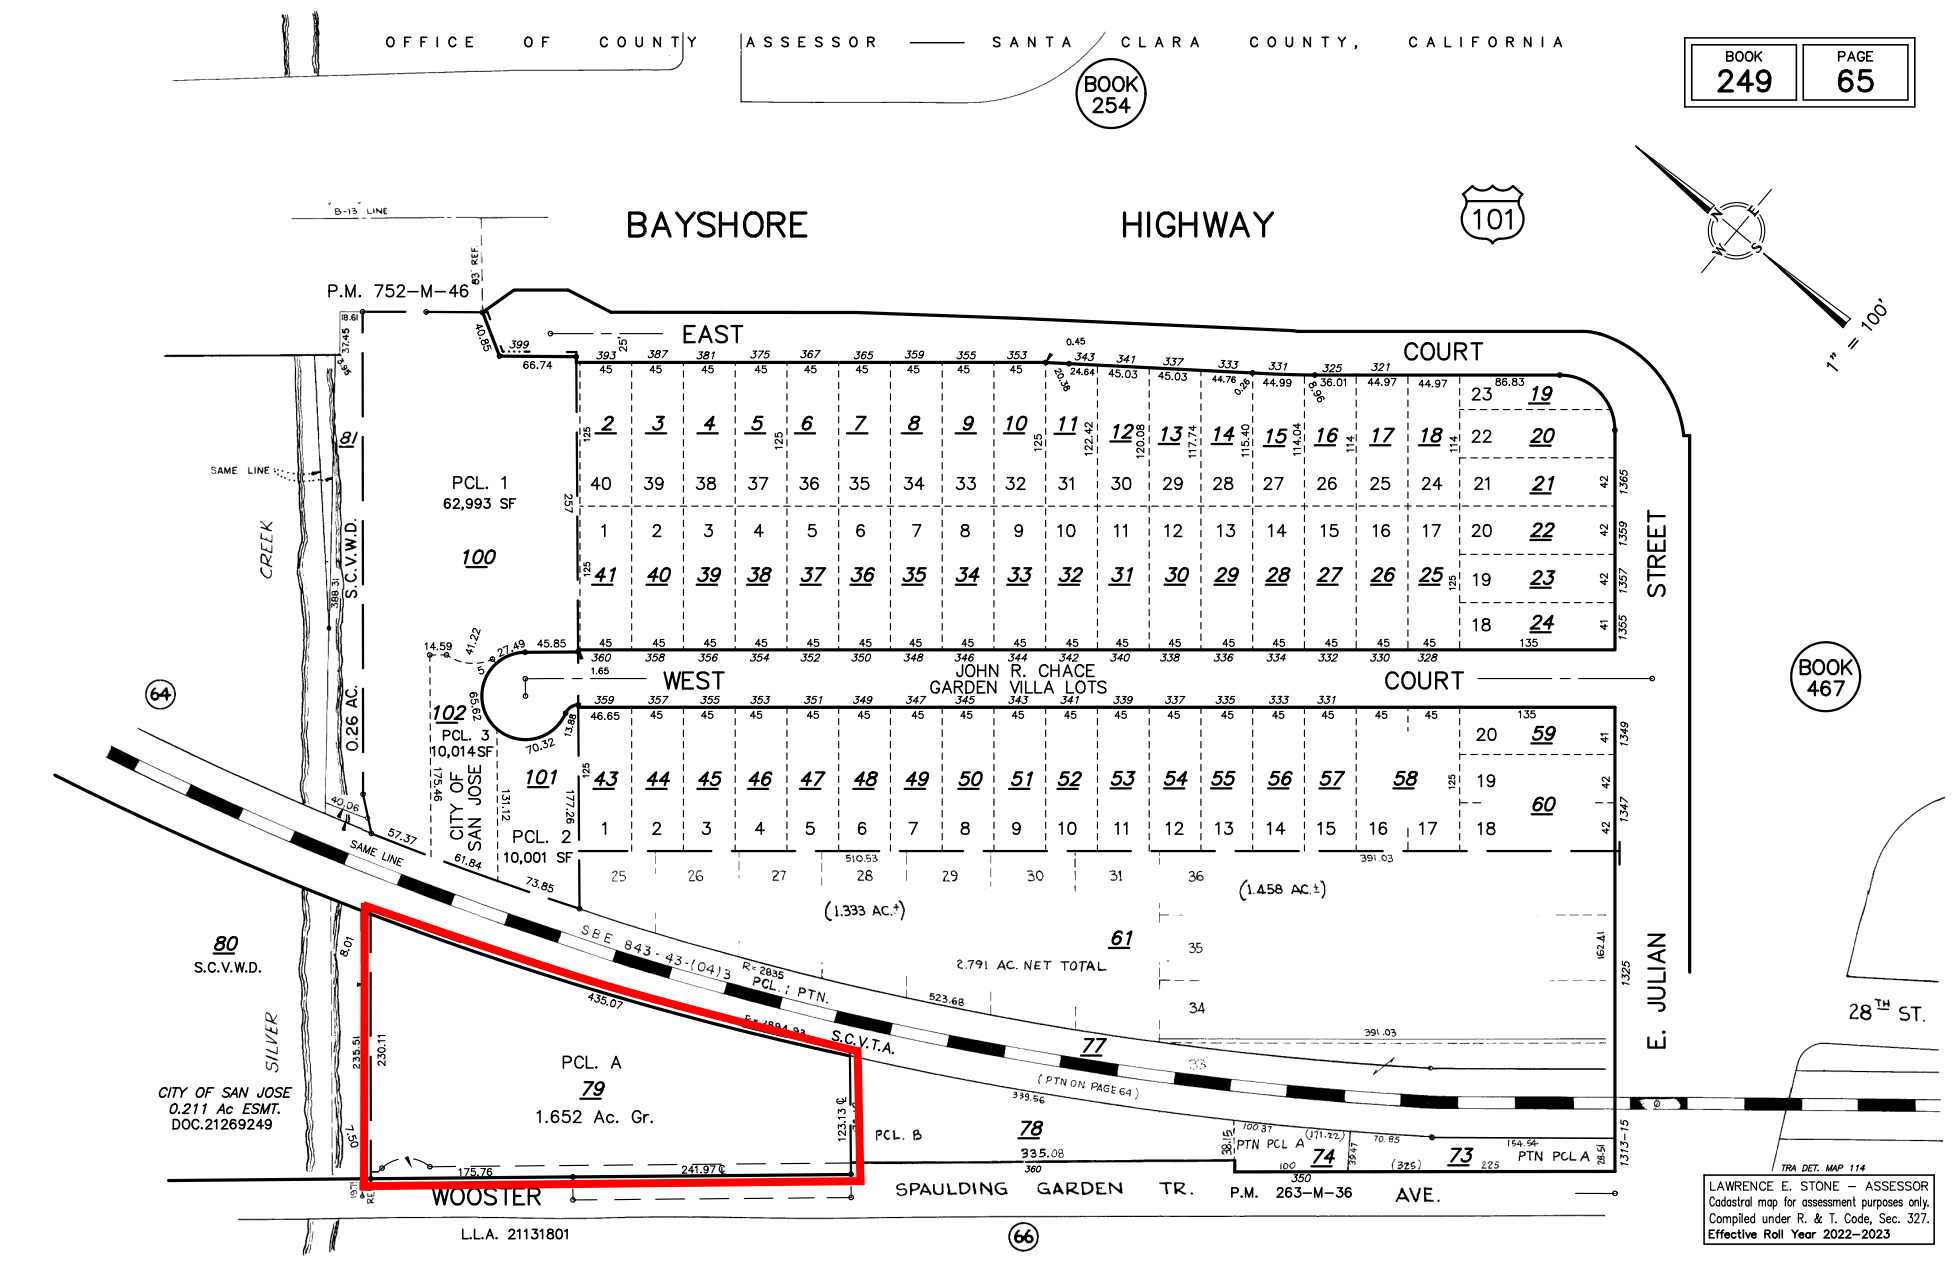
\includegraphics[width=\textwidth]{Assessor-Info/discovery-prep-plat-map-249-65}\\ %chktex 8
    \footnotesize{Santa Clara County Assessor's Office (n.d.). [Plat Map]. Retrieved 23 Dec 2022 from  \url{https://tinyurl.com/discovery-prep-plat-map}}.
\end{figure}

\begin{table}[hbt]
  \SingleSpacing%
  \caption[Discovery Prep: Taxable Amount of Assessed Propery]{\textit{Discovery Prep: Taxable Amount of Assessed Property}}\label{tab:discovery-prep-taxable-amount}
  \begin{tabular}{llll}
    \toprule
    Year & Land        & Improvements & Total Assessed Value \\
    \midrule
    2022 & \$2,414,563 & \$4,289,318  & \$6,703,881 \\
    2021 & \$2,367,219 & \$4,205,214  & \$6,572,433 \\
    2020 & \$2,342,947 & \$4,162,095  & \$6,505,042 \\
    \bottomrule
  \end{tabular}
\end{table}

\begin{figure}[hbt]
  \caption[Discovery Prep Satellite Photo]{\textit{Discovery Prep Satellite Photo}}\label{fig:discovery-prep-sat-photo}
  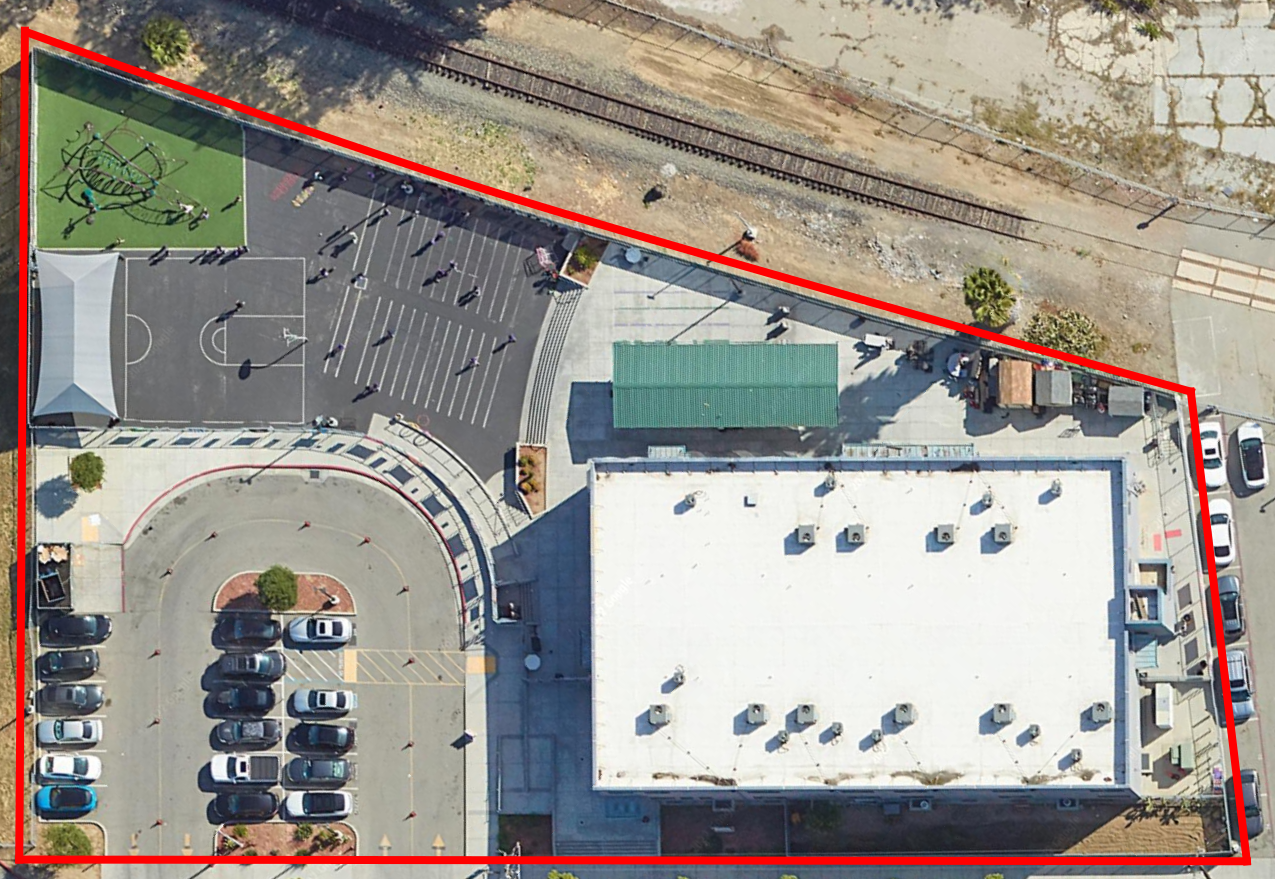
\includegraphics[width=\textwidth]{Satellite-Photos/discovery-prep-sat-photo}\\ %chktex 8
  \footnotesize{Google. (n.d). [Google Earth image]. Retrieved 23 Dec 2022 from \url{https://tinyurl.com/discovery-prep-v2}.}
\end{figure}

%%%%%%%%%%%%%%%%%%%%%%%%%%%%%%%%%%%%%%%%%%%%%%%%%%%%%%%%%%%%%%%%%%%%%%%%%%%%%%%%%%%%%%%%%%%%%%%%%%%%%%%%%%%%%%%%%%%%%%%%%

\clearpage
\section{Mosaic}\label{sec:mosaic-info}
\begin{table}[htb]
  \SingleSpacing%
  \caption[Mosaic: Property Information]{\textit{Mosaic: Property Information}}\label{tab:mosaic-prop-info}
  \begin{tabular}{ll}
    \toprule
    Property Address      & 950 Owsley Ave, San José, CA 95122 \\
    Assessor's Parcel No. & 477–34–088 \\
    Size                  & 1.011ac \\
    Date of Last Sale     & 24 May 2011 \\
    \bottomrule
  \end{tabular}
\end{table}

\begin{figure}[hbt]
    \caption[Mosaic Plat Map]{\textit{Mosaic Plat Map}}\label{fig:mosaic-plat-map}
    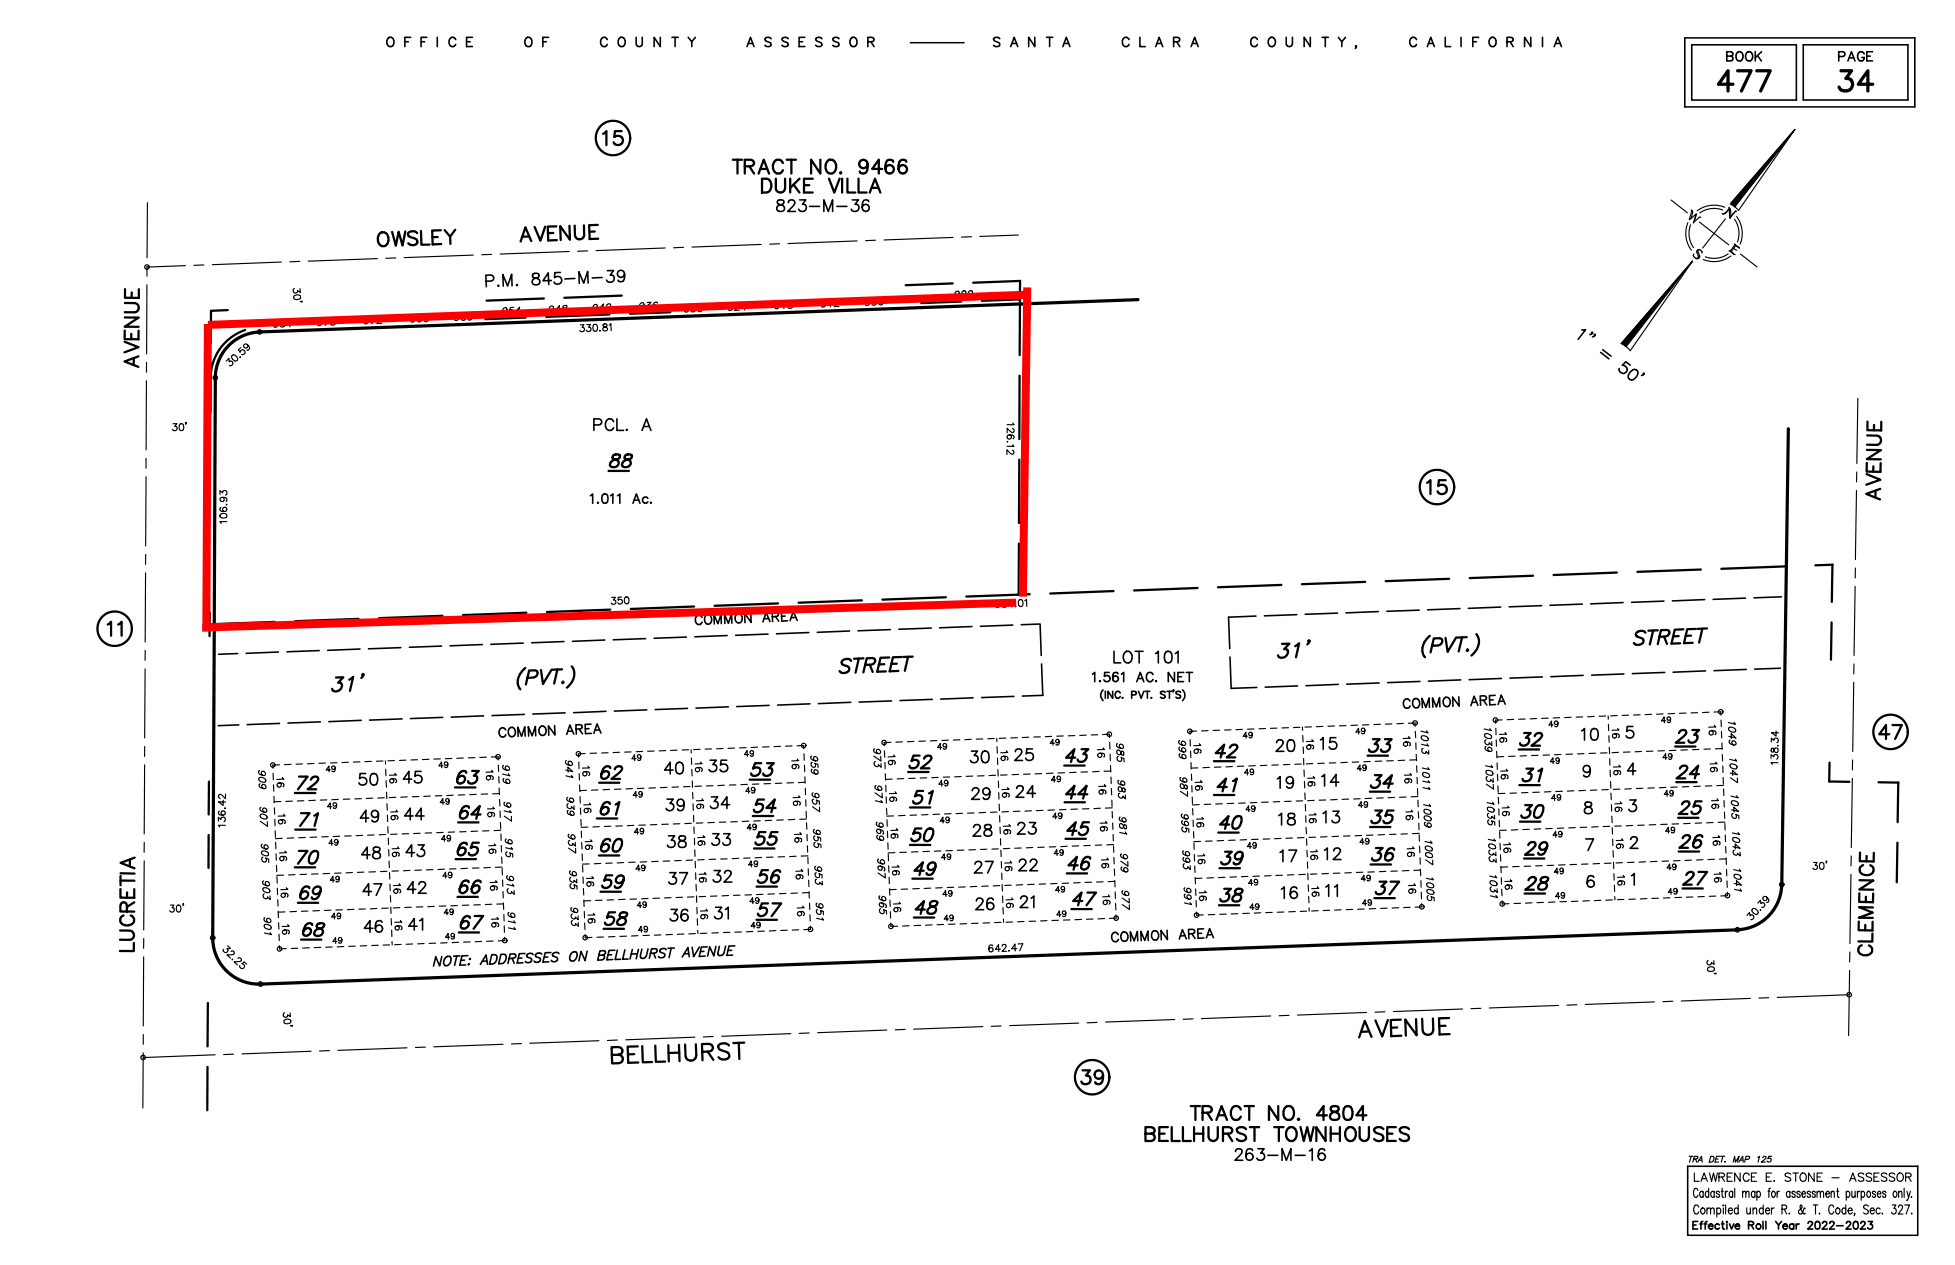
\includegraphics[width=\textwidth]{Assessor-Info/mosaic-plat-map-477-34}\\ %chktex 8
    \footnotesize{Santa Clara County Assessor's Office (n.d.). [Plat Map]. Retrieved 23 Dec 2022 from  \url{https://tinyurl.com/mosaic-plat-map}}.
\end{figure}

\begin{table}[hbt]
  \SingleSpacing%
  \caption[Mosaic: Taxable Amount of Assessed Propery]{\textit{Mosaic: Taxable Amount of Assessed Property}}\label{tab:mosaic-taxable-amount}
  \begin{tabular}{llll}
    \toprule
    Year & Land        & Improvements & Total Assessed Value \\
    \midrule
    2022 & \$1,851,242 & \$4,971,161 & \$6,822,403 \\
    2021 & \$1,814,944 & \$4,873,688 & \$6,688,632 \\
    2020 & \$1,796,334 & \$4,823,715 & \$6,620,049 \\
    \bottomrule
  \end{tabular}
\end{table}

\begin{figure}[hbt]
  \caption[Mosaic Satellite Photo]{\textit{Mosaic Satellite Photo}}\label{fig:mosaic-sat-photo}
  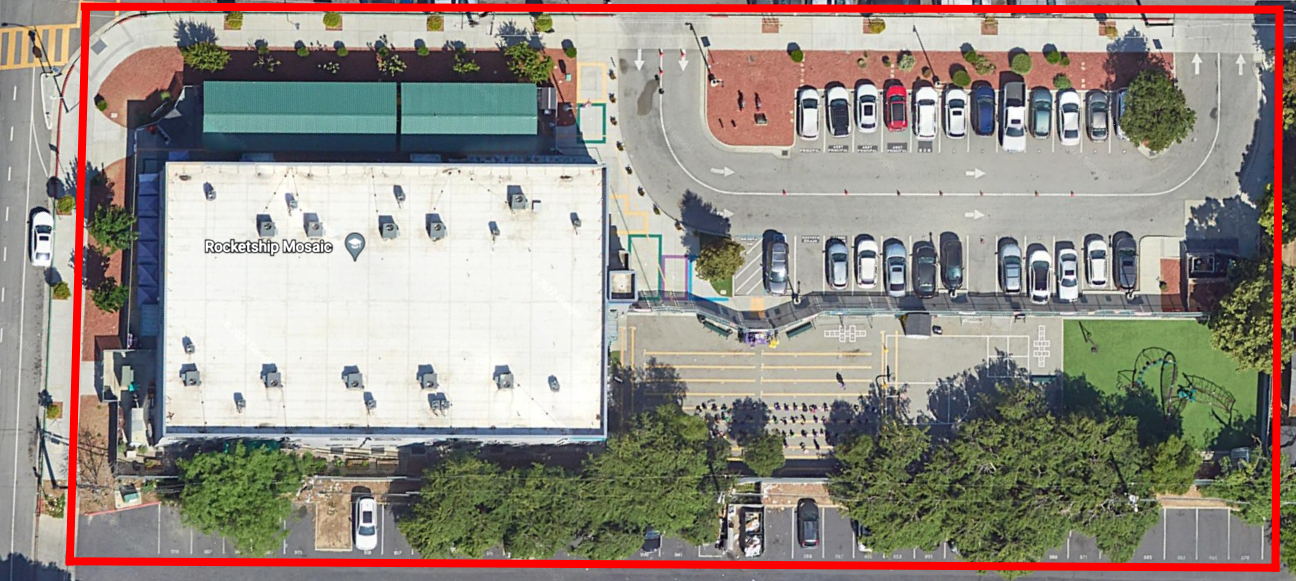
\includegraphics[width=\textwidth]{Satellite-Photos/mosaic-sat-photo}\\ %chktex 8
  \footnotesize{Google. (n.d). [Google Earth image]. Retrieved 23 Dec 2022 from \url{https://tinyurl.com/mosaic-v3}.}
\end{figure}

%%%%%%%%%%%%%%%%%%%%%%%%%%%%%%%%%%%%%%%%%%%%%%%%%%%%%%%%%%%%%%%%%%%%%%%%%%%%%%%%%%%%%%%%%%%%%%%%%%%%%%%%%%%%%%%%%%%%%%%%%

\clearpage
\section{Brilliant Minds}\label{sec:brilliant-minds-info}

\begin{table}[htb]
  \SingleSpacing%
  \caption[Brilliant Minds: Property Information]{\textit{Brilliant Minds: Property Information}}\label{tab:brilliant-minds-prop-info}
  \begin{tabular}{ll}
    \toprule
    Property Address      & \multirow[t]{2}{3in}{2960 Story Rd, San Jose, CA 95127 \\
    2962 Story Rd, San Jose, CA 95127} \\\\
    Assessor's Parcel No. & 488-03-003 \\
    Size                  & 1.223ac \\
    Date of Last Sale     & 11 Feb 2014\\
    \bottomrule
  \end{tabular}\\\newline
  \noindent\footnotesize{Note: Brilliant Minds occupies a single parcel, along with two churches. It appears to have its own buildings, but shares the single parking lot. The size of the parcel is 2.446ac, and arbitrarily, half has been allocated to Rocketship Brilliant Minds.}  
\end{table}


\begin{figure}[t]
  \centering
  \caption[Brilliant Minds Plat Map]{\textit{Brilliant Minds Plat Map}}\label{fig:brilliant-minds-plat-map}
  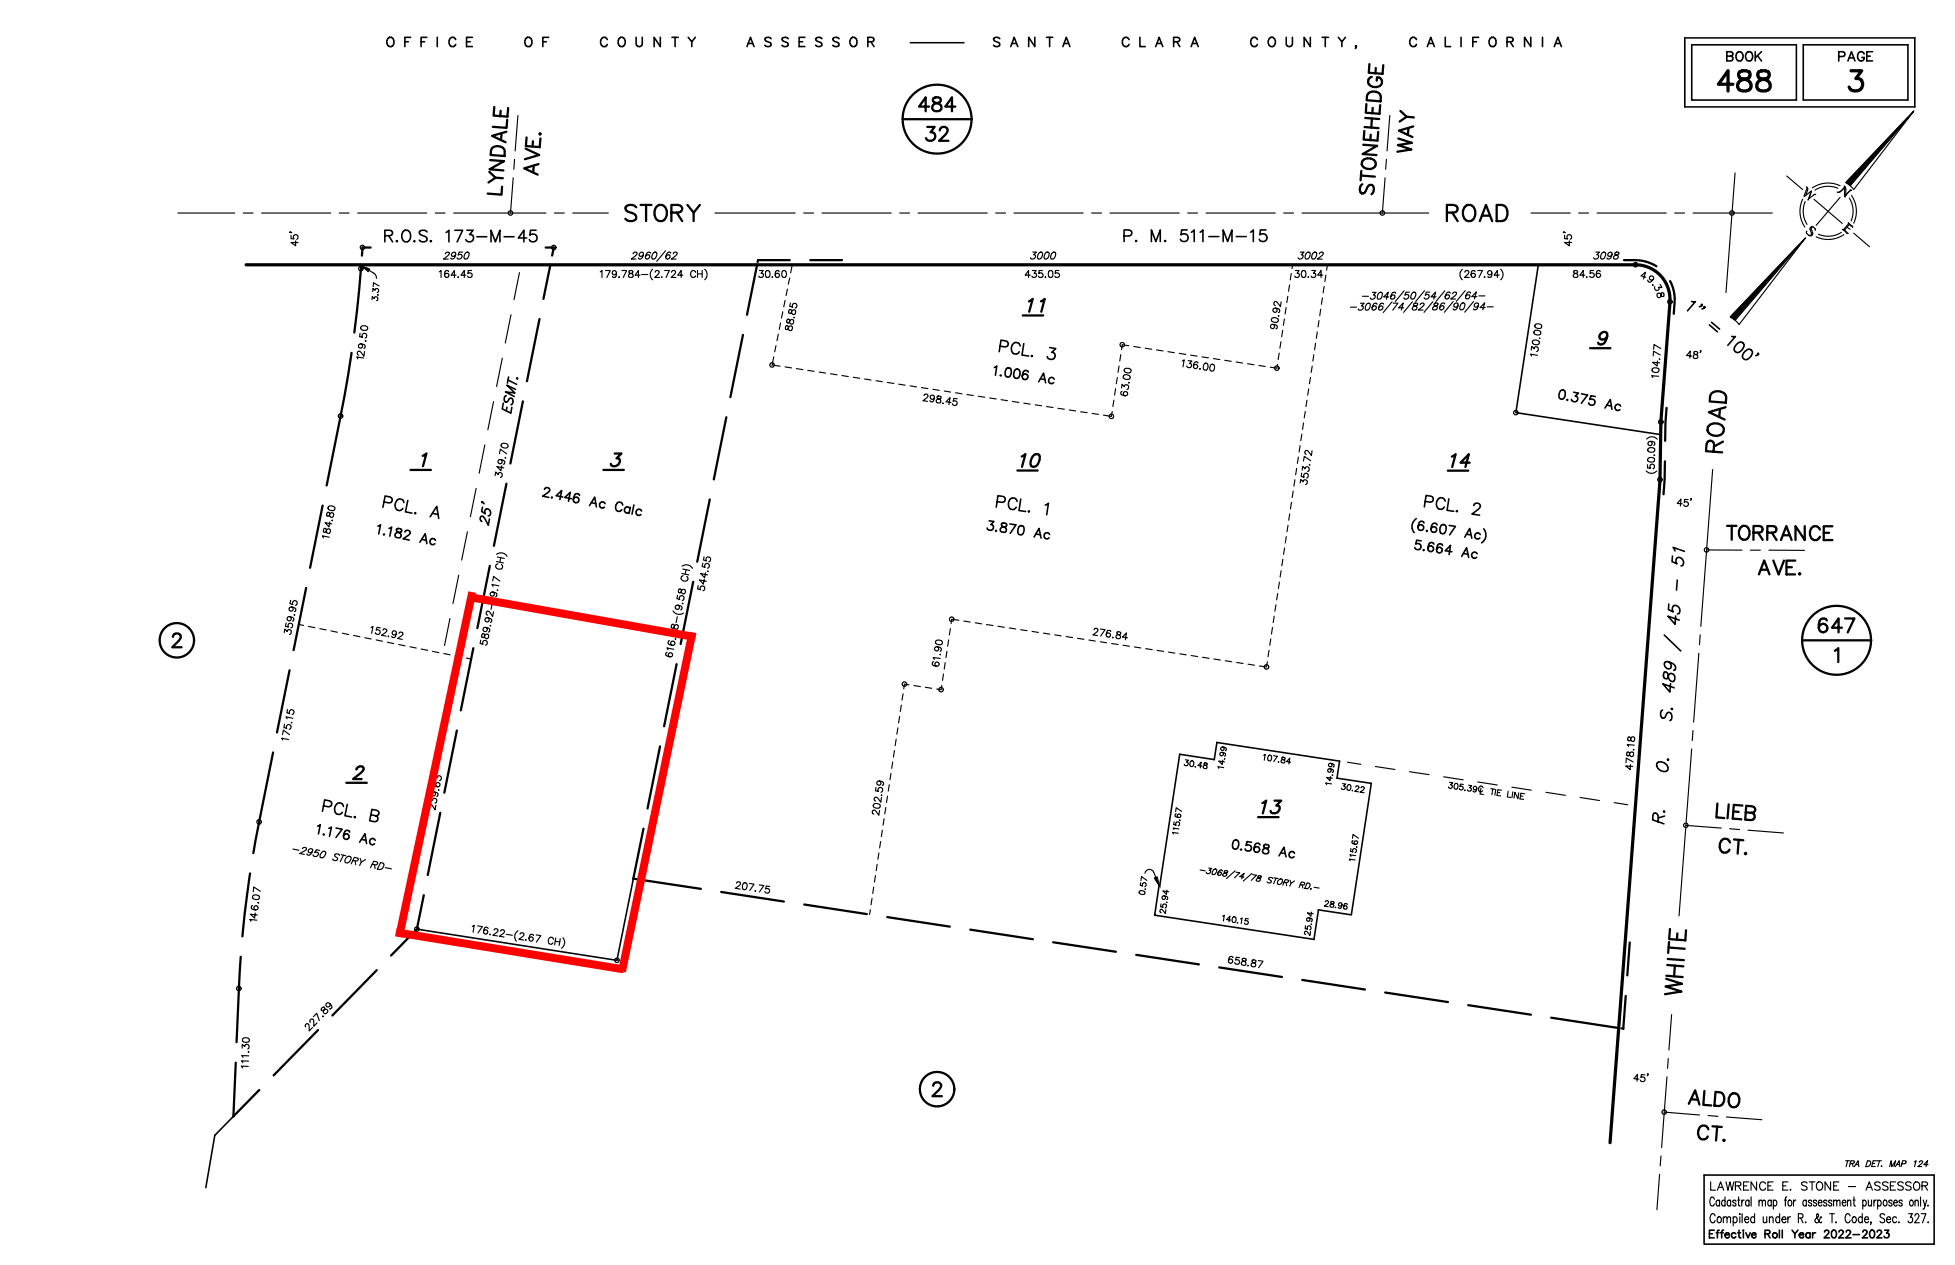
\includegraphics[width=\textwidth]{Assessor-Info/brilliant-minds-plat-map-488-03}\\ %chktex 8
  \footnotesize{Santa Clara County Assessor's Office (n.d.). [Plat Map]. Retrieved 23 Dec 2022 from  \url{https://tinyurl.com/brilliant-minds-plat-map}}.
\end{figure}

\begin{table}[hbt]
\SingleSpacing%
  \caption[Brilliant Minds: Taxable Amount of Assessed Propery]{\textit{Brilliant Minds: Taxablekk Amount of Assessed Property}}\label{tab:brilliant-minds-taxable-amount}
  \begin{tabular}{llll}
    \toprule
   Year  & Land        & Improvements & Total Assessed Value \\
    \midrule
    2022 & \$8,630,187 & \$4,218,635  & \$12,848,822 \\
    2021 & \$8,460,968 & \$4,135,917  & \$12,596,885 \\
    2020 & \$8,374,212 & \$4,093,509  & \$12,467,721 \\
    \bottomrule
  \end{tabular}
\end{table}

\begin{figure}[hbt]
  \centering
  \caption[Brilliant Minds Satellite Photo]{\textit{Brilliant Minds Satellite Photo}}\label{fig:brilliant-minds-sat-photo}
  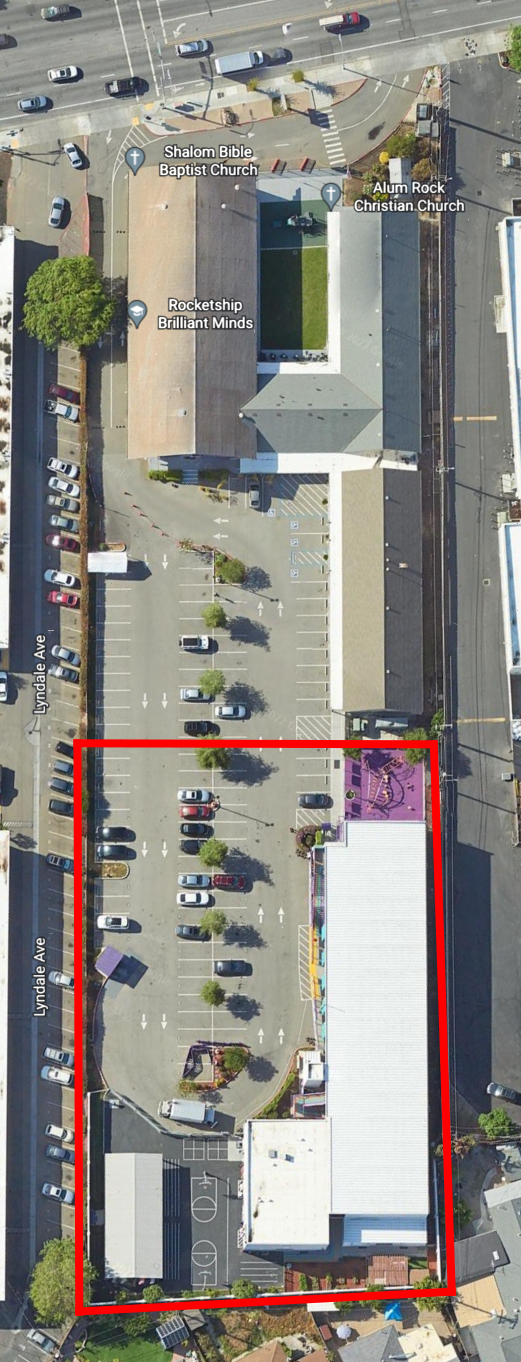
\includegraphics[height=0.9\textheight]{Satellite-Photos/brilliant-minds-sat-photo}\\ %chktex 8
  \footnotesize{Google. (n.d). [Google Earth image]. Retrieved 23 Dec 2022 from \url{https://tinyurl.com/brilliant-minds-v2}.}
\end{figure}

%%%%%%%%%%%%%%%%%%%%%%%%%%%%%%%%%%%%%%%%%%%%%%%%%%%%%%%%%%%%%%%%%%%%%%%%%%%%%%%%%%%%%%%%%%%%%%%%%%%%%%%%%%%%%%%%%%%%%%%%%

\clearpage
\section{Alma Academy}\label{sec:alma-academy-info}
\begin{table}[htb]
  \SingleSpacing%
  \caption[Alma Academy: Property Information]{\textit{Alma Academy}: Property Information}\label{tab:alma-academy-prop-info}
  \begin{tabular}{ll}
    \toprule
    Property Address      & 198 West Alma Ave, San José, CA 95110 \\
    Assessor's Parcel No. & 434–22–{097,098,099,100,119,132} \\
    Size                  & 0.551ac \\
    Date of Last Sale     & 12 Apr 2012 \\
    \bottomrule
  \end{tabular}
\end{table}

\begin{figure}[hbt]
    \caption[Alma Academy Plat Map]{\textit{Alma Academy Plat Map}}\label{fig:alma-academy-plat-map}
    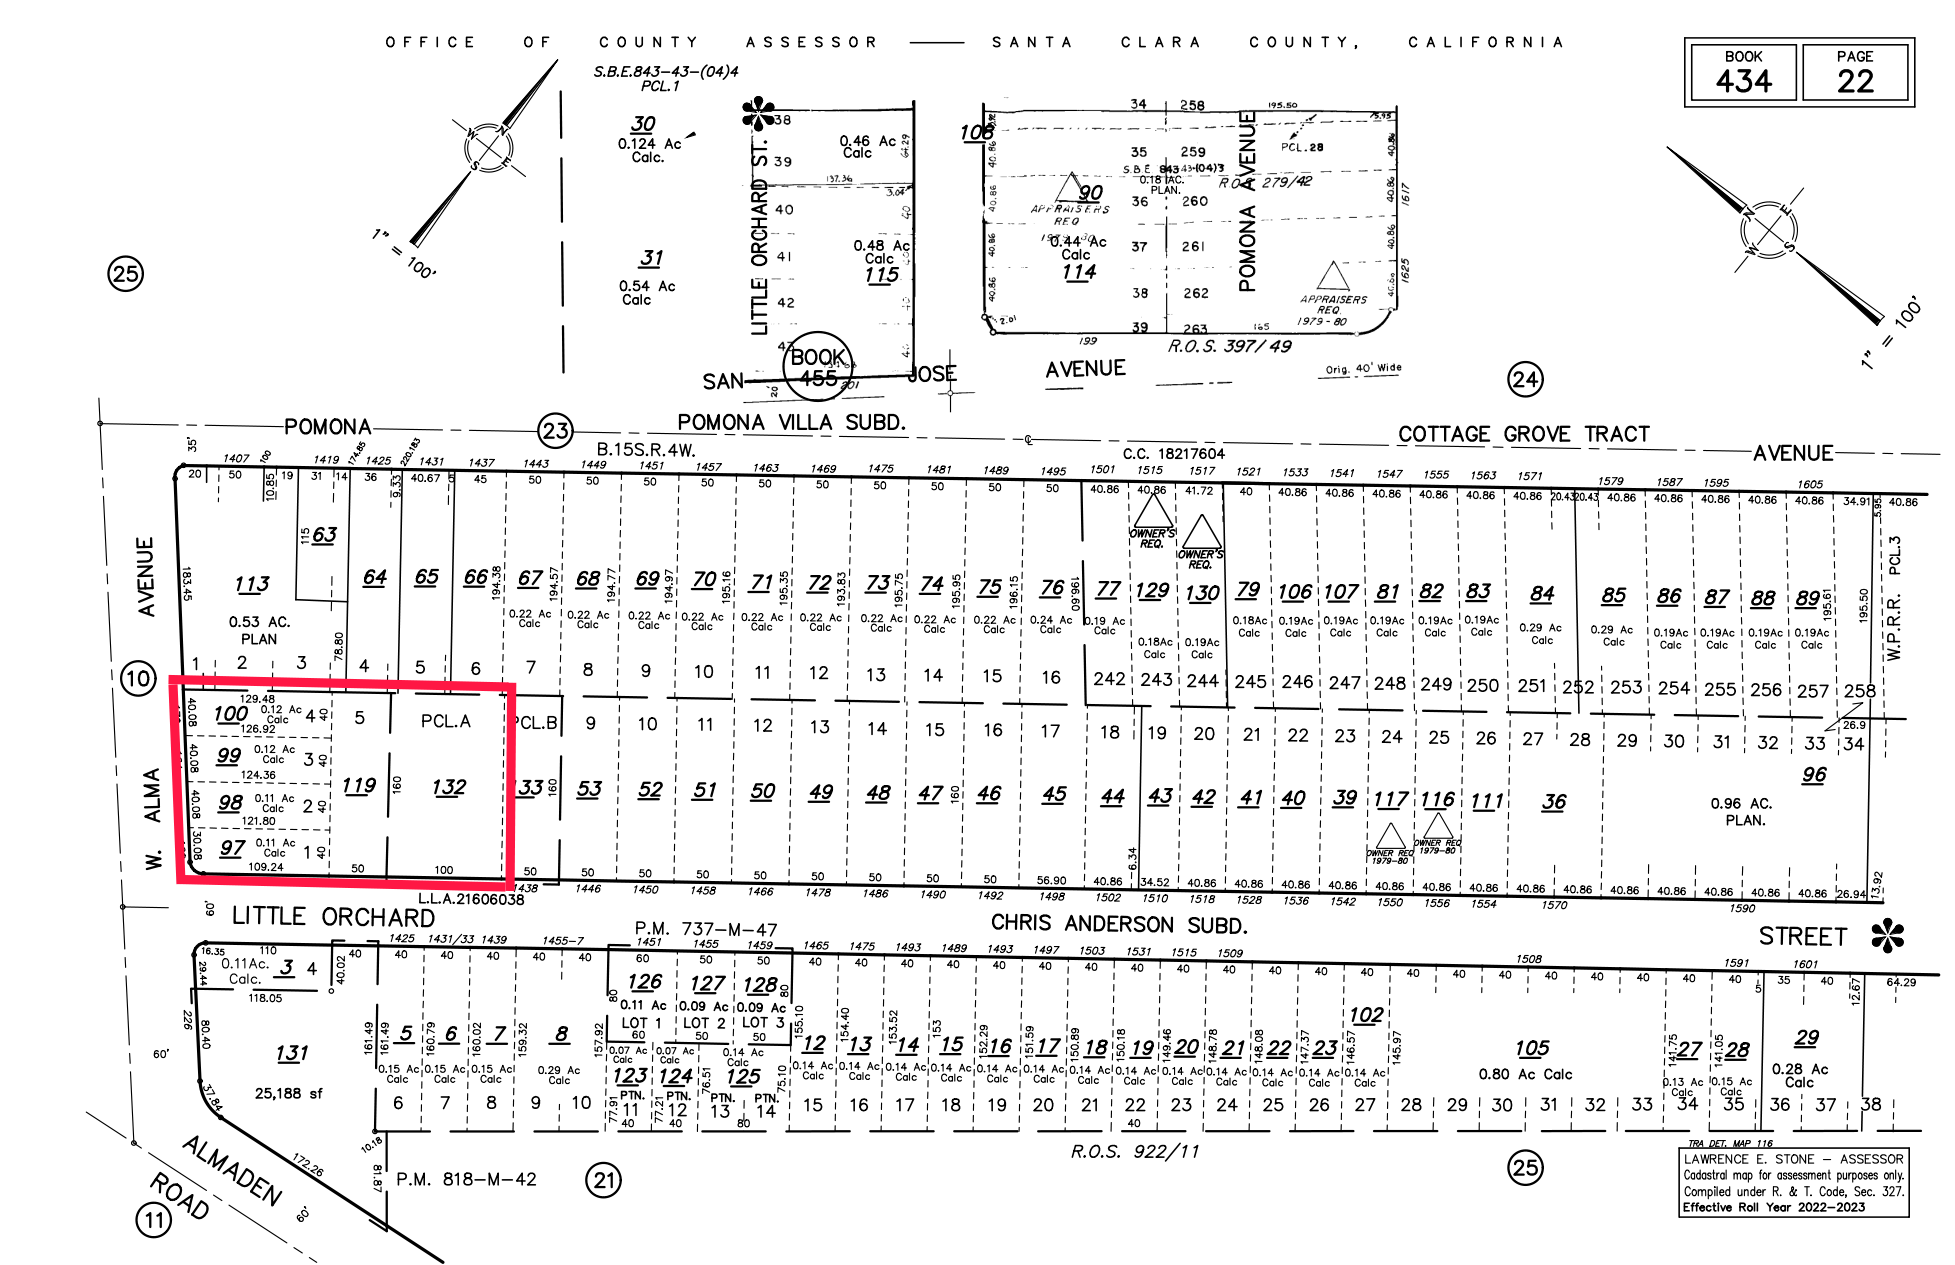
\includegraphics[width=0.9\textwidth]{Assessor-Info/alma-academy-plat-map-434-22}\\ %chktex 8
    \footnotesize{Santa Clara County Assessor's Office (n.d.). [Plat Map]. Retrieved 03 Jan 2023 from  \url{https://tinyurl.com/alma-academy-plat-map-v2}.}
\end{figure}

\begin{table}[hbt]
  \SingleSpacing%
  \caption[Alma Academy: Taxable Amount of Assessed Propery]{\textit{Alma Academy: Taxable Amount of Assessed Property}}\label{tab:alma-academy-taxable-amount}
  \begin{tabular}{llll}
    \toprule
    Year & Land        & Improvements & Total Assessed Value \\
    \midrule
    2022 & \$1,615,598 & \$0          & \$1,615,598 \\
    2021 & \$1,583,932 & \$0          & \$1,583,932 \\
    2020 & \$1,567,686 & \$0          & \$1,567,686 \\
    \bottomrule
  \end{tabular}\\\newline
  \noindent\footnotesize{Note: Rocketship Alma Academy comprises adjacent six parcels, so the assessed value indicated in this table is the sum of all six parcels.}
\end{table}

\begin{figure}[hbt]
  \centering
  \caption[Alma Academy Satellite Photo]{\textit{Alma Academy Satellite Photo}}\label{fig:alma-academy-sat-photo}
  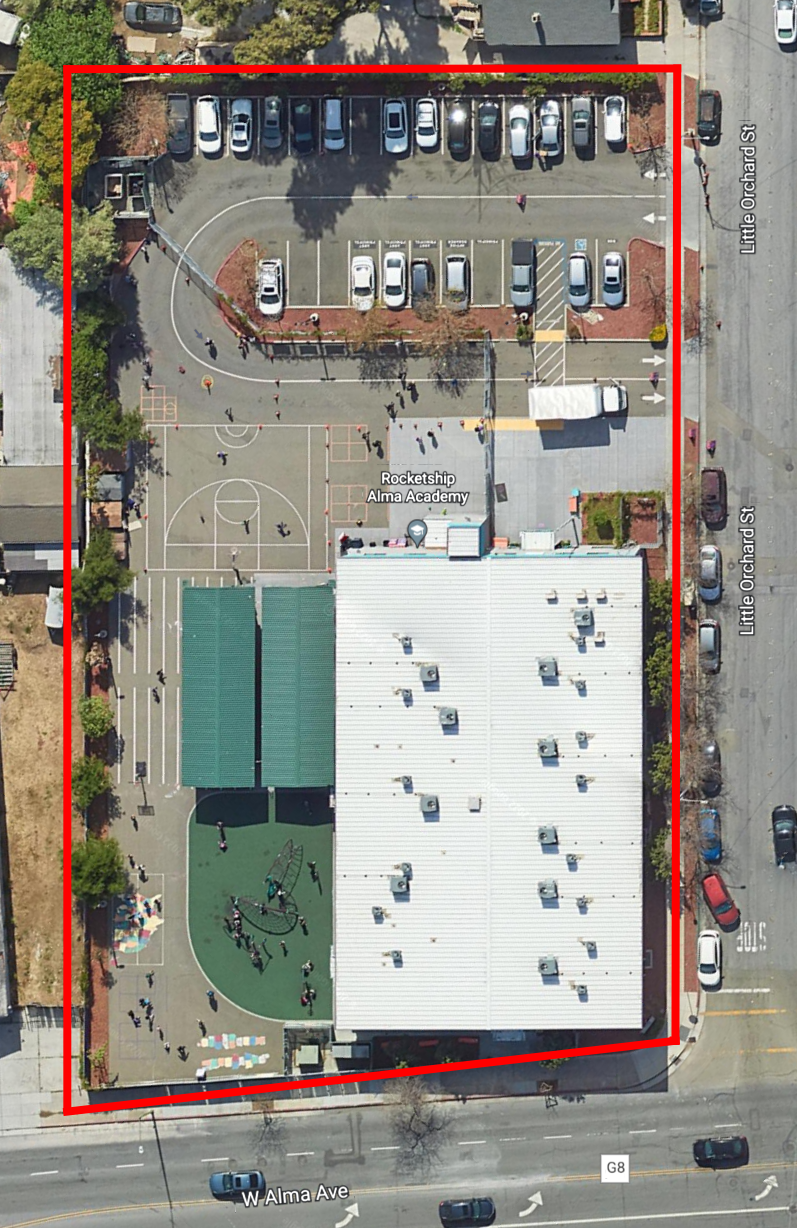
\includegraphics[height=0.667\textheight]{Satellite-Photos/alma-academy-sat-photo}\\ %chktex 8
  \footnotesize{Google. (n.d). [Google Earth image]. Retrieved 03 Jan 2023 from \url{https://tinyurl.com/alma-academy}.}
\end{figure}

%%%%%%%%%%%%%%%%%%%%%%%%%%%%%%%%%%%%%%%%%%%%%%%%%%%%%%%%%%%%%%%%%%%%%%%%%%%%%%%%%%%%%%%%%%%%%%%%%%%%%%%%%%%%%%%%%%%%%%%%%

\clearpage
\section{Spark Academy}\label{sec:spark-academy-info}

\begin{table}[htb]
  \SingleSpacing%
  \caption[Spark Academy: Property Information]{\textit{Spark Academy: Property Information}}\label{tab:spark-academy-prop-info}
  \begin{tabular}{ll}
    \toprule
    Property Address      & 683 Sylvandale Ave San José, CA 95111 \\
    Assessor's Parcel No. & [494-72-001] \\
    Size                  & approx. 1ac \\
    Date of Last Sale     & [01 Jun 2012]\\
    \bottomrule
  \end{tabular}\\
  \noindent\footnotesize{Note: Spark Academy has a land lease from the Franklin McKinley School District, so the figures above enclosed in brackets are those of the Franklin McKinley School District.}  
\end{table}

\begin{figure}[hbt]
    \caption[Spark Academy Plat Map]{\textit{Spark Academy Plat Map}}\label{fig:spark-academy-plat-map}
    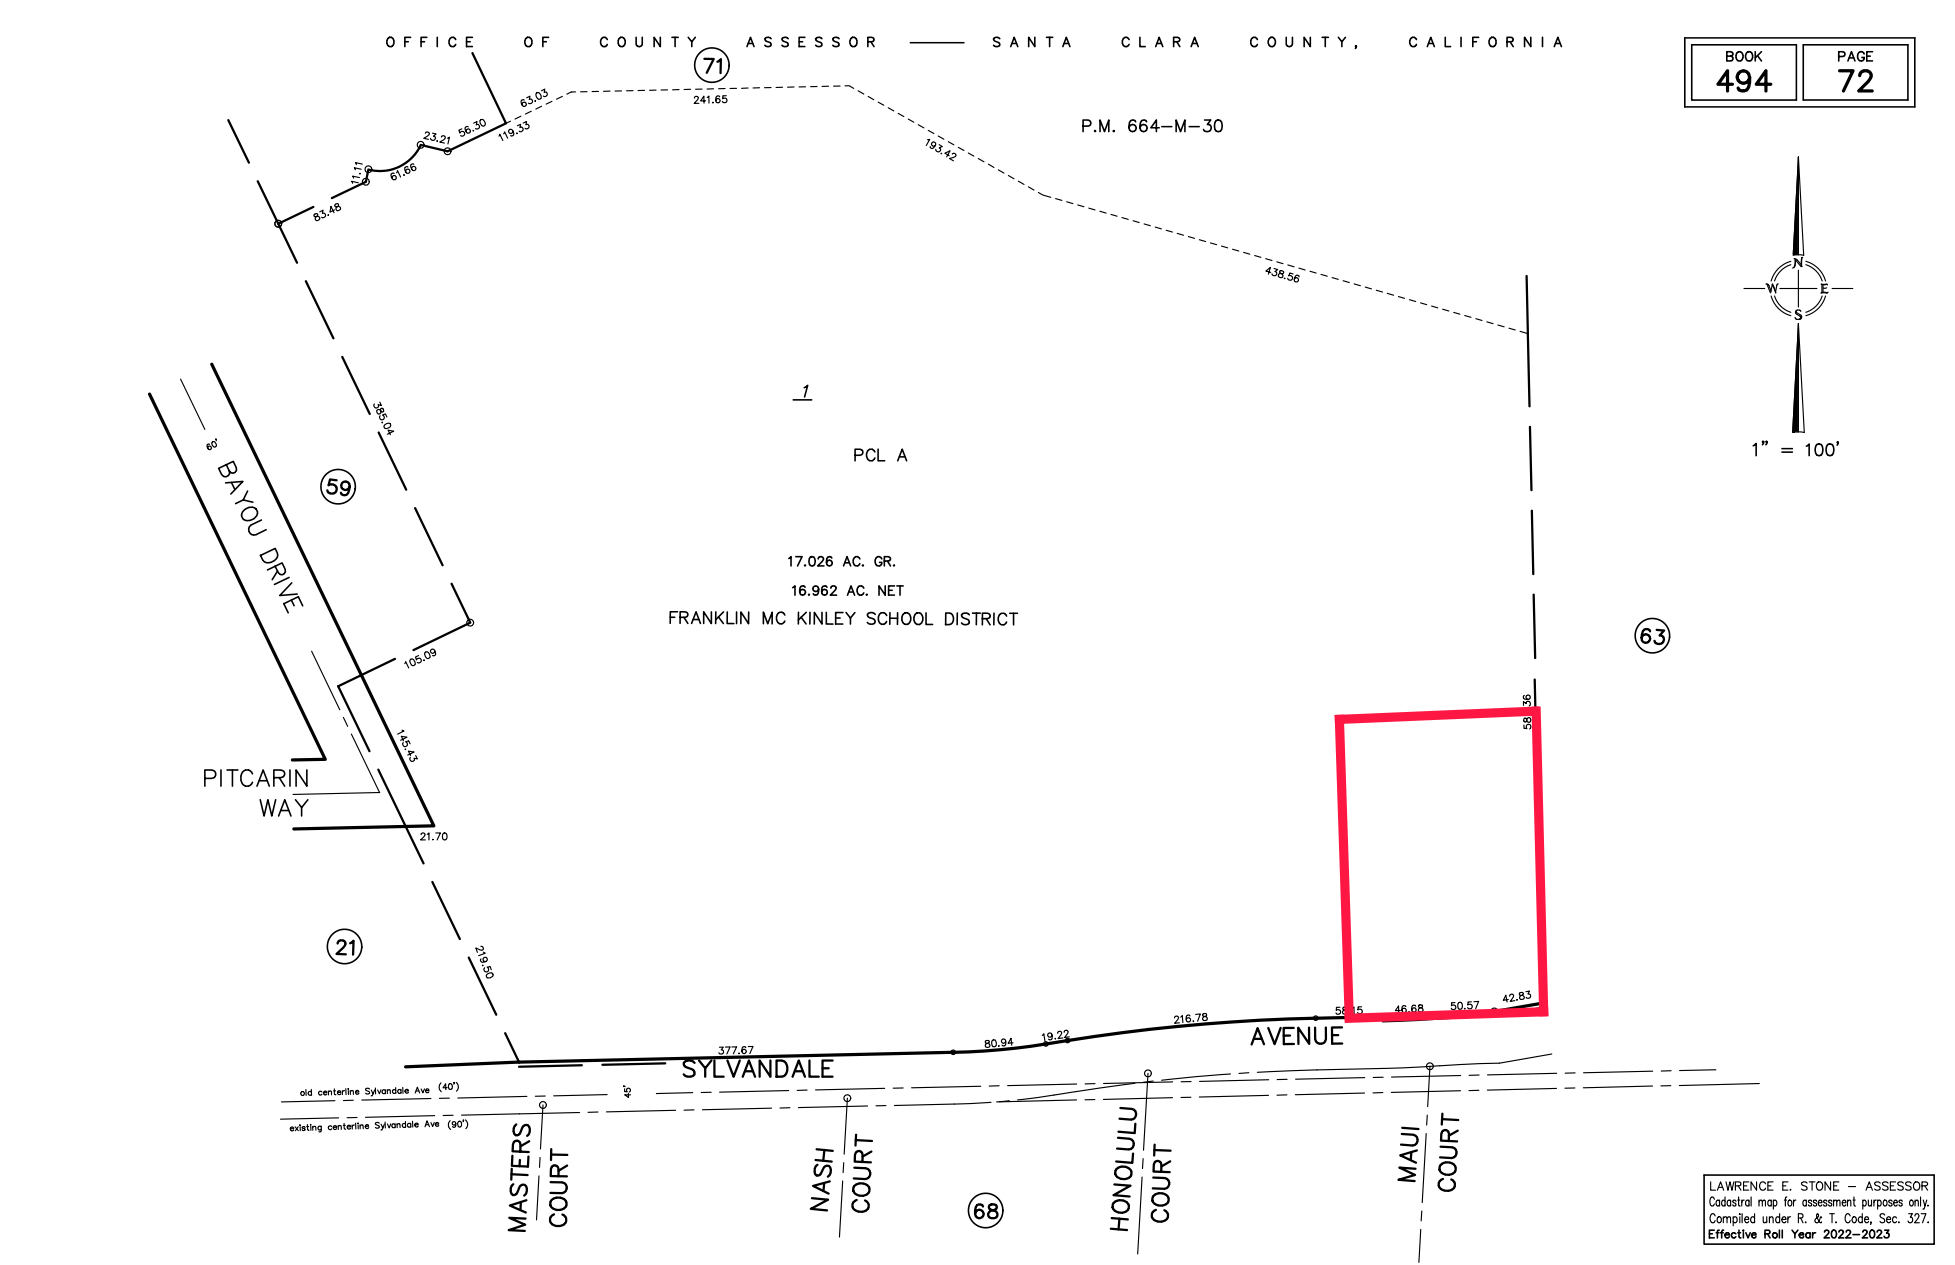
\includegraphics[width=\textwidth]{Assessor-Info/spark-academy-plat-map-494-72}\\ %chktex 8
    \footnotesize{Santa Clara County Assessor's Office (n.d.). [Plat Map]. Retrieved 07 Jan 2023 from  \url{https://tinyurl.com/spark-academy-plat-map}}.
    
    \noindent\footnotesize{Note: The outline is approximate.}
  \end{figure}

\begin{table}[hbt]
  \SingleSpacing%
  \caption[Spark Academy: Taxable Amount of Assessed Propery]{\textit{Spark Academy: Taxable Amount of Assessed Property}}\label{tab:spark-academy-taxable-amount}
  \begin{tabular}{llll}
    \toprule
    Year & Land        & Improvements & Total Assessed Value \\
    \midrule
    2022 & \$0         & \$0          & \\
    2021 & \$0         & \$0          & \\
    2020 & \$0         & \$0          & \\
    \bottomrule
  \end{tabular}\\
  \noindent\footnotesize{Note: As noted above, Spark Academy leases its land from the Franklin McKinley School District. Since public school districts are exempt from property taxes, all the taxable amounts in this table are listed as \$0.}
\end{table}

\begin{figure}[hbt]
  \centering
  \caption[Spark Academy Satellite Photo] {\textit{Spark Academy Satellite Photo}}\label{fig:spark-academy-sat-photo}
  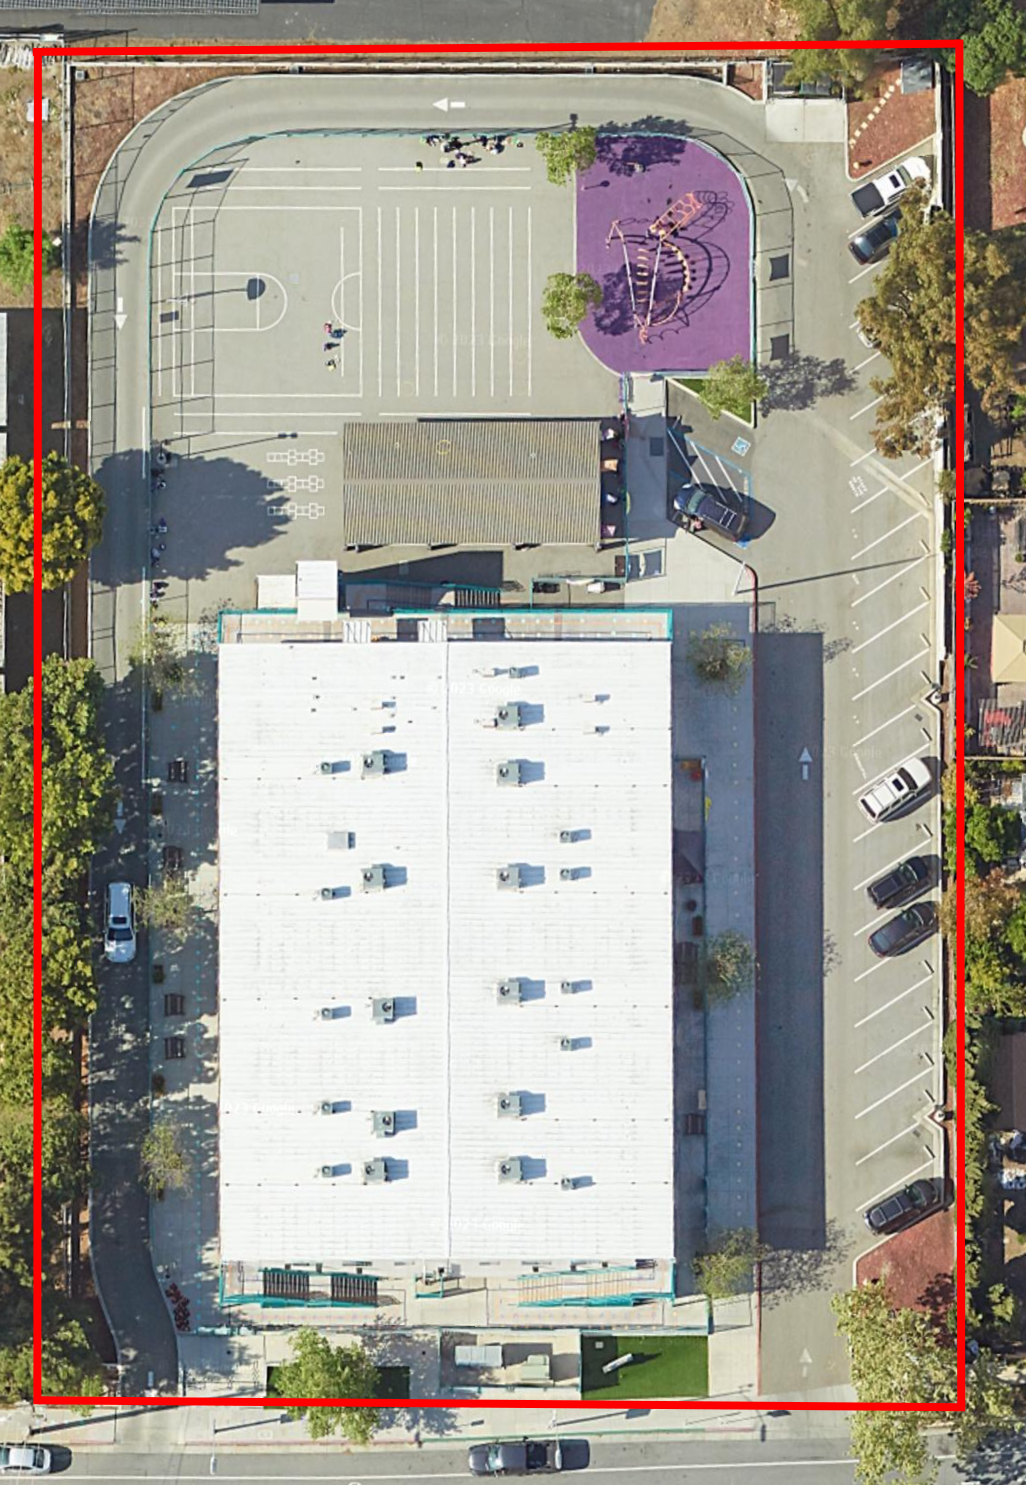
\includegraphics[height=0.6\textheight]{Satellite-Photos/spark-academy-sat-photo}\\ %chktex 8
  \footnotesize{Google. (n.d). [Google Earth image]. Retrieved 07 Jan 2023 from \url{https://tinyurl.com/spark-academy}.}
  \noindent\footnotesize{Note: The outline is approximate.}
\end{figure}

%%%%%%%%%%%%%%%%%%%%%%%%%%%%%%%%%%%%%%%%%%%%%%%%%%%%%%%%%%%%%%%%%%%%%%%%%%%%%%%%%%%%%%%%%%%%%%%%%%%%%%%%%%%%%%%%%%%%%%%%%

\clearpage
\section{Fuerza }\label{sec:fuerza-info}

\begin{table}[htb]
  \SingleSpacing%
  \caption[Fuerza: Property Information]{\textit{Fuerza: Property Information}}\label{tab:fuerza-prop-info}
  \begin{tabular}{ll}
    \toprule
    Property Address      & 70 S. Jackson Ave, San José, CA 95116 \\
    Assessor's Parcel No. & 484–41–162 \\
    Size                  & 1.35ac \\
    Date of Last Sale     & 02 Feb 2018 \\
    \bottomrule
  \end{tabular}
\end{table}

\begin{figure}[hbt]
    \caption[Fuerza Plat Map]{\textit{Fuerza Plat Map}}\label{fig:fuerza-plat-map}
    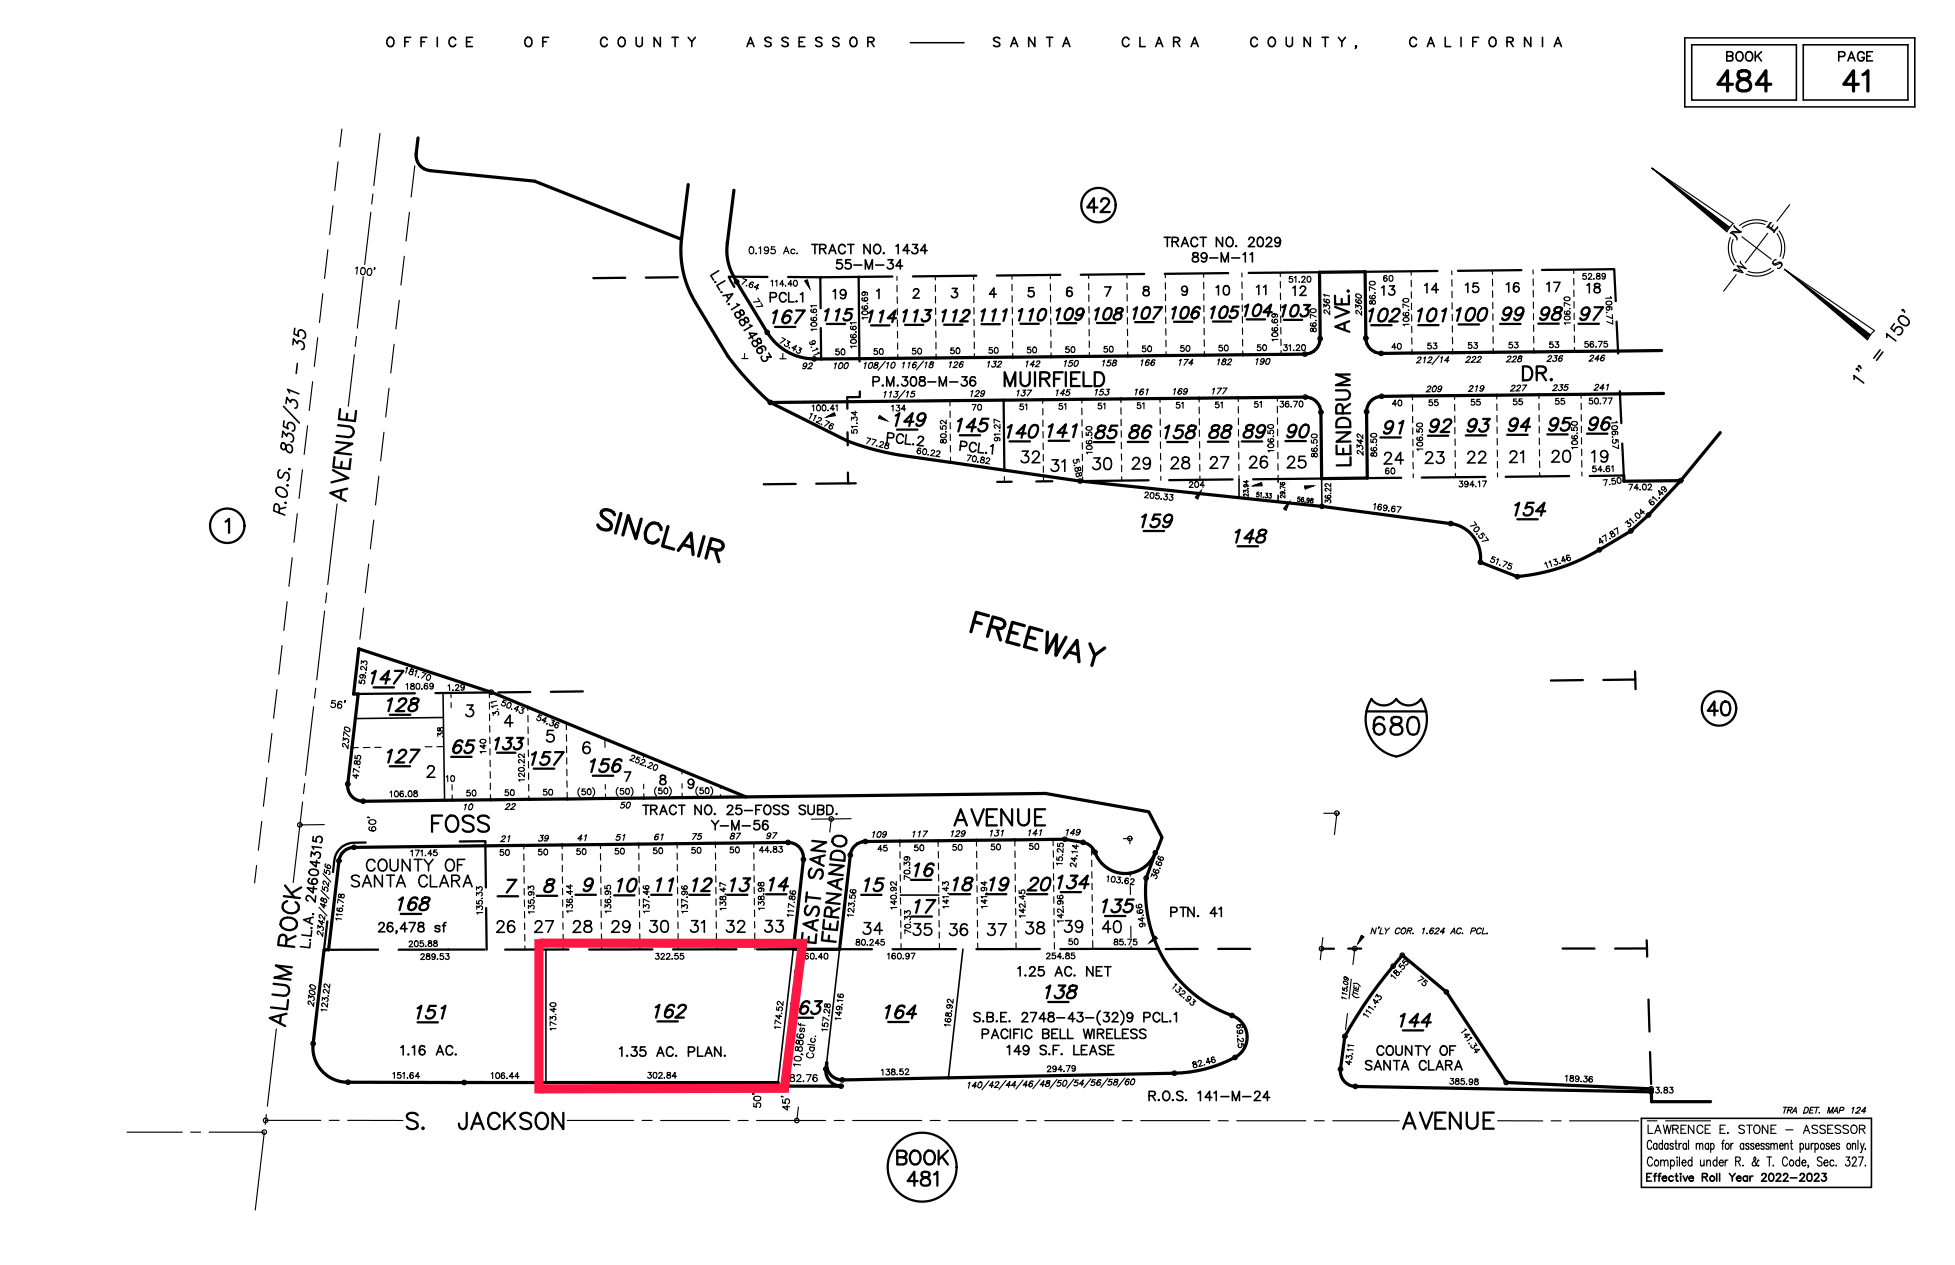
\includegraphics[width=\textwidth]{Assessor-Info/fuerza-plat-map-484-41}\\ %chktex 8
    \footnotesize{Santa Clara County Assessor's Office (n.d.). [Plat Map]. Retrieved 07 Jan 2023 from  \url{https://tinyurl.com/fuerza-plat-map}}.
\end{figure}

\begin{table}[hbt]
  \SingleSpacing%
  \caption[Fuerza: Taxable Amount of Assessed Propery]{\textit{Fuerza: Taxable Amount of Assessed Property}}\label{tab:fuerza-taxable-amount}
  \begin{tabular}{llll}
    \toprule
    Year & Land        & Improvements & Total Assessed Value \\
    \midrule
    2022 & \$2,656,862 & \$937,117    & \$3,593,979 \\
    2021 & \$2,604,767 & \$918,743    & \$3,523,510 \\
    2020 & \$2,578,059 & \$909,323    & \$3,487,382 \\
    \bottomrule
  \end{tabular}
\end{table}

\begin{figure}[hbt]
  \caption[Fuerza Satellite Photo]{\textit{Fuerza Satellite Photo}}\label{fig:fuerza-sat-photo}
  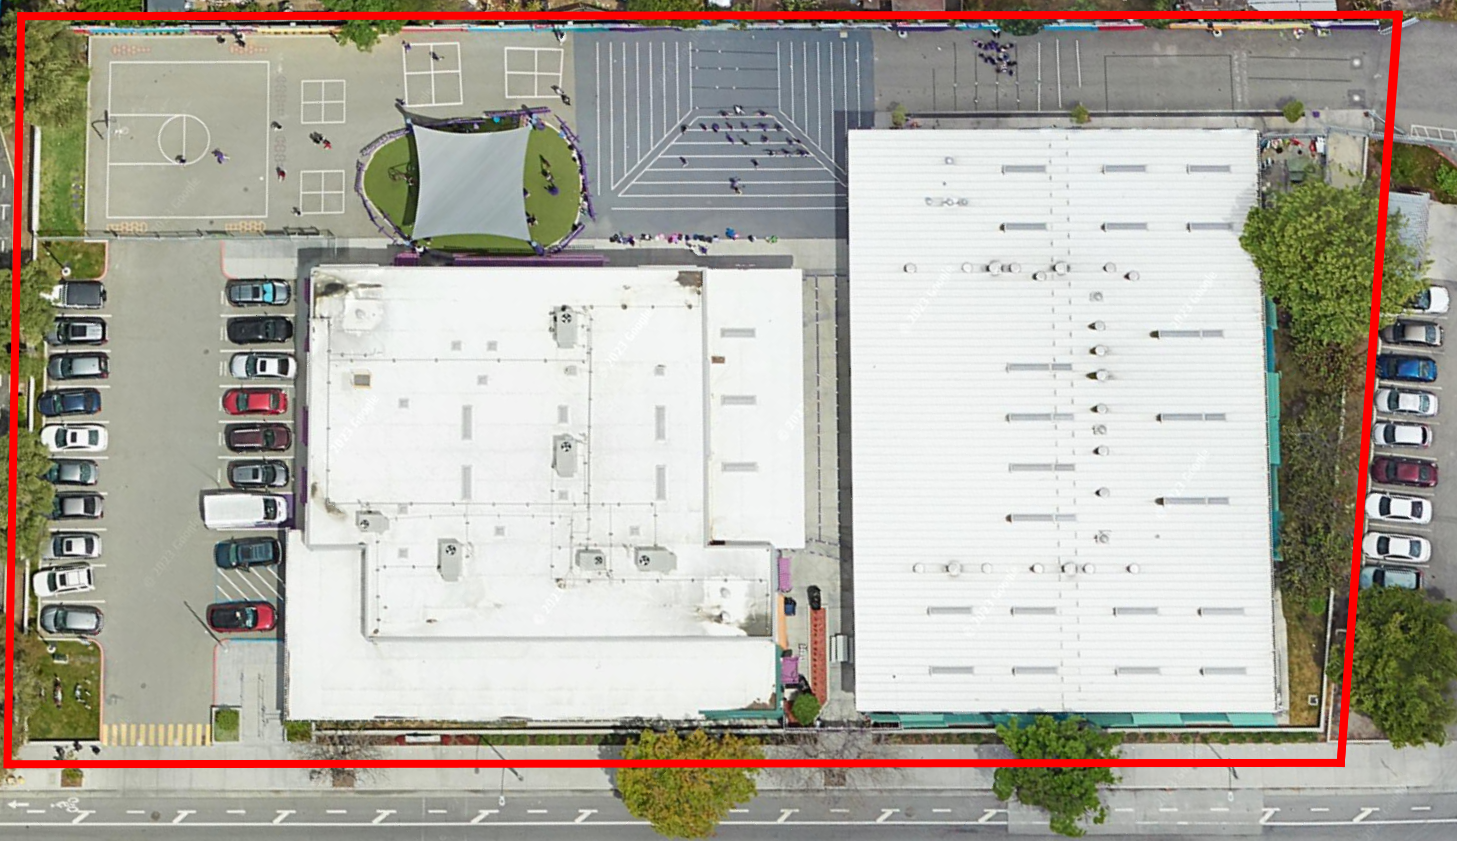
\includegraphics[width=\textwidth]{Satellite-Photos/fuerza-sat-photo}\\ %chktex 8
  \footnotesize{Google. (n.d). [Google Earth image]. Retrieved 07 Jan 2023 from \url{https://tinyurl.com/fuerza-v2}.}
\end{figure}

%%%%%%%%%%%%%%%%%%%%%%%%%%%%%%%%%%%%%%%%%%%%%%%%%%%%%%%%%%%%%%%%%%%%%%%%%%%%%%%%%%%%%%%%%%%%%%%%%%%%%%%%%%%%%%%%%%%%%%%%%

\clearpage
\section{Rising Stars}\label{sec:rising-stars-info}

\begin{table}[htb]
  \SingleSpacing%
  \caption[Rising Stars: Property Information]{\textit{Rising Stars: Property Information}}\label{tab:rising-stars-prop-info}
  \begin{tabular}{ll}
    \toprule
    Property Address      & 3173 Senter Road, San José, CA 95111 \\
    Assessor's Parcel No. & 494–01–027 \\
    Size                  & 1.58ac \\
    Date of Last Sale     & 01 Dec 2016 \\
    \bottomrule
  \end{tabular}
\end{table}

\begin{figure}[hbt]
    \caption[Rising Stars Plat Map]{\textit{Rising Stars Plat Map}}\label{fig:rising-stars-plat-map}
    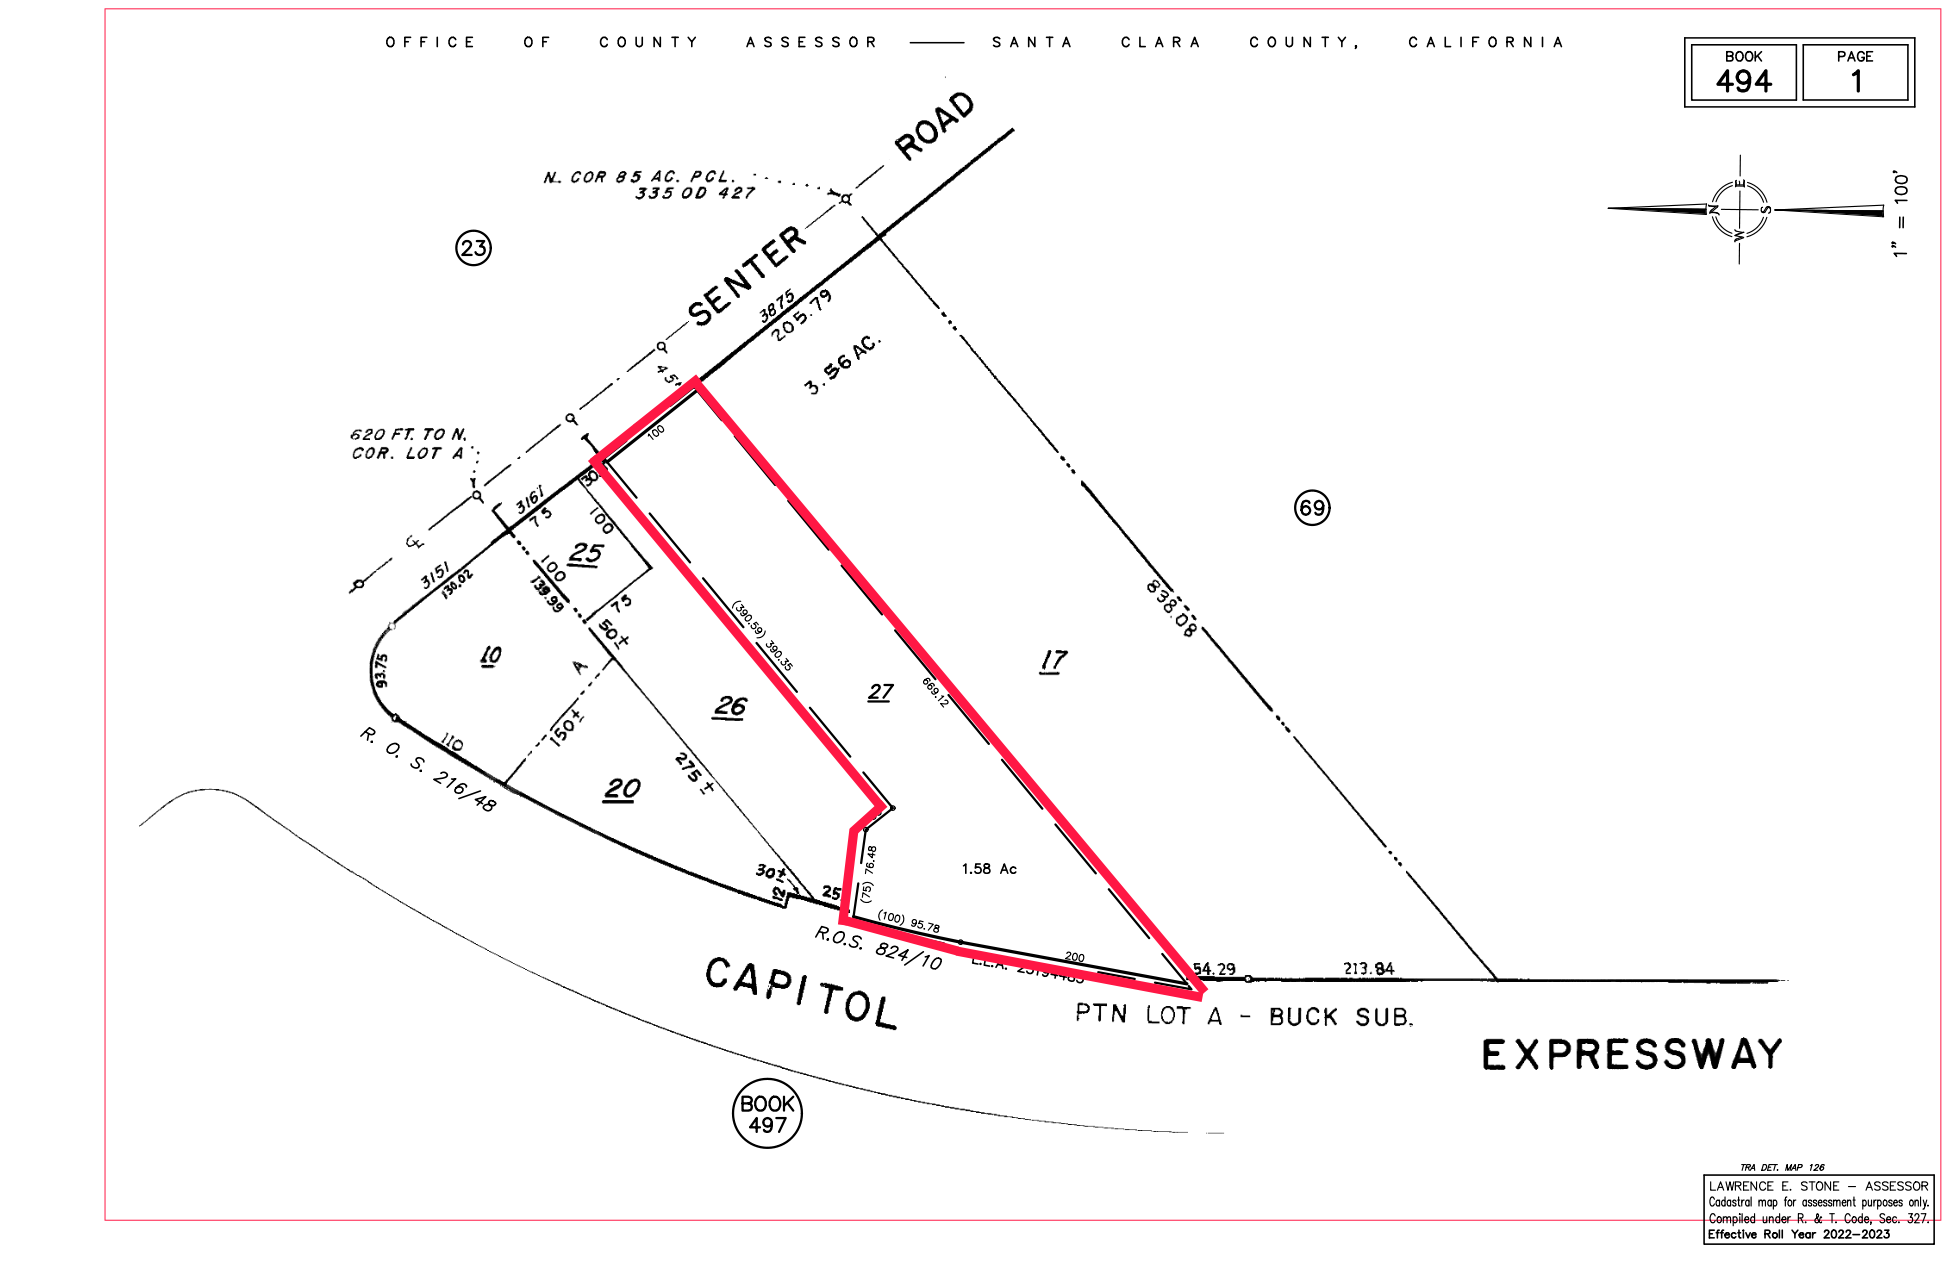
\includegraphics[width=\textwidth]{Assessor-Info/rising-stars-plat-map-494-01}\\ %chktex 8
    \footnotesize{Santa Clara County Assessor's Office (n.d.). [Plat Map]. Retrieved 07 Jan 2023 from  \url{https://tinyurl.com/rising-stars-plat-map}}.
\end{figure}

\begin{table}[hbt]
  \SingleSpacing%
  \caption[Rising Stars: Taxable Amount of Assessed Propery]{\textit{Rising Stars: Taxable Amount of Assessed Property}}\label{tab:rising-stars-taxable-amount}
  \begin{tabular}{llll}
    \toprule
    Year & Land        & Improvements & Total Assessed Value \\
    \midrule
    2022 & \$2,997,872 & \$12,139,470 & \$15,137,342 \\
    2021 & \$2,939,091 & \$11,901,442 & \$12,139,470 \\
    2020 & \$2,908,955 & \$11,779,408 & \$14,688,363 \\
    \bottomrule
  \end{tabular}
\end{table}

\begin{figure}[hbt]
  \centering
  \caption[Rising Stars Satellite Photo]{\textit{Rising Stars Satellite Photo}}\label{fig:rising-stars-sat-photo}
  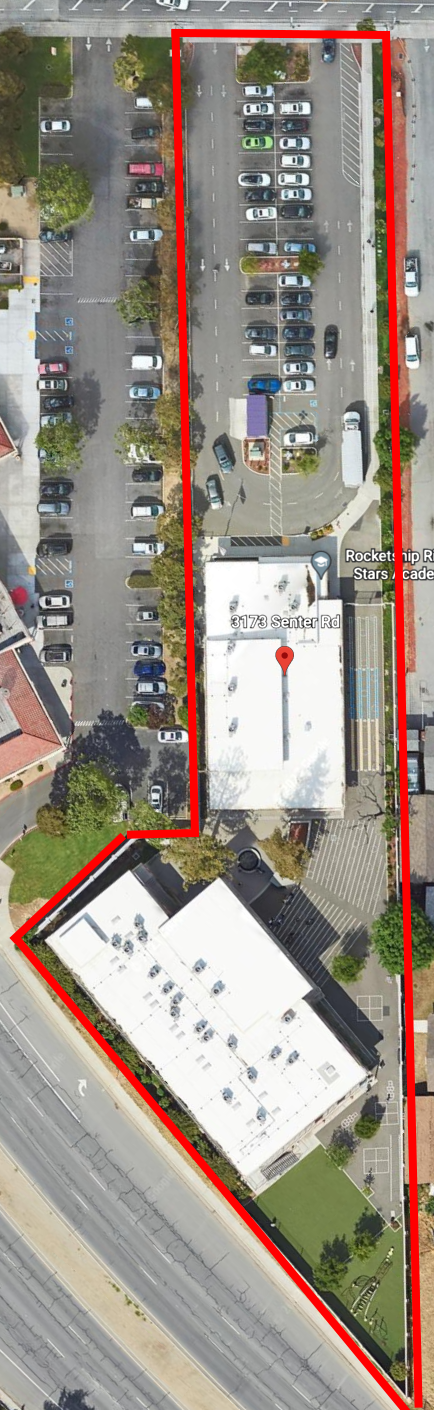
\includegraphics[height=0.667\textheight]{Satellite-Photos/rising-stars-sat-photo}\\ %chktex 8
  \footnotesize{Google. (n.d). [Google Earth image]. Retrieved 07 Jan 2023 from \url{https://tinyurl.com/rising-stars-v2}.}
\end{figure}

%%% Local Variables:
%%% mode: latex
%%% TeX-master: "Rocketship_Education-An_Exploratory_Public_Policy_Case_Study"
%%% End:
